\chapter{Problem Description}
The essence of a collaborative, distributed system is that every node performs tasks for other nodes.
With open systems, where every one can join, an unsolved problem is how to prevent nodes
from only consuming and not contributing to the system.
Our work is an important first step forward in solving this problem without a central system
and a need to use force.

In this chapter the problem will be described of how to decide to perform a task for a peer.
In such a way that prevents that peer from freeloading.
The problem will first be explained in a simplified form.
Using this simplification, the problem will be transformed gradually
to the real world problem faced in distributed systems today.

\section{Freeriding public goods}
The problem in collaborative, distributed systems is nodes freeriding public goods.
Nodes are participants in the system and the free goods are the willingness of these participants to help others.
The field of game theory has studied for decades this problem of how
participants can decide to cooperate with a peer or not\cite{Hardin-Tragedy}.
Deciding not to help can prevent freeriding.
The minimal form of this problem is with only two participants.
This form is called the Prisoner's Dilemma
and we will explain this dilemma\cite{Nowak-PrisonerDilemma}\cite{Lai-Incentives}.

Participants can help each other at a cost, a negative utility,
but the recipient of the help will receive a beneficial utility from the help.
The benefit received is greater than the cost and is denoted by $R$ for reward.
But if one participant chooses to not help the other participant,
then he will still receive a beneficial utility and at no cost, $T$ for temptation.
The participant that provided the aid will now receive no benefit and only incur a cost $C$.
If both participants choose to not help each other,
then they will both receive a penalty $P$, which is higher then the cost of helping each other.
One participant can be called participant A and the other participant B.
The utility received by A and B based upon their decision can be seen in Table \ref{tab:pd-um}.

\begin{table}
\center
	\begin{tabular}{l|ll}
	A\textbackslash B       & cooperate  & defect     \\ \hline
	cooperate & $R_A /R_B$ & $T_A /C_B$ \\
	defect    & $T_A /C_B$ & $P_A /P_B$
	\end{tabular}
\caption{Prisoner's Dilemma utility matrix}
\label{tab:pd-um}
\end{table}

This dilemma can be repeated several times with the same participants and is the Iterated Prisoner's Dilemma.
Each time both participants will have to decide if they will help the other participant.
A rational participant wants to receive maximum benefit at a minimal cost.
The participant will follow a strategy that he believes will achieve this.
At first it might seem that a participant will always choose to defect,
because it will never incur a cost and receive maximal benefit.
But the other participant will be reluctant to help a participant if the aid is never returned.
Simple strategies, like tit-for-tat or win-stay, lose-shift, suffice in the Iterated Prisoner's Dilemma
and will perform well\cite{Nowak-Cooperation}.

The participants receive direct reciprocity from the other participant\cite{Nowak-Cooperation}.
Direct reciprocity is displayed abstractly in Figure \ref{fig:direct-reciprocity}.
Participant A helps participant B and in returns receives help.
This help will be extended in the future under the assumption it is returned.

\begin{figure}
	\centerline{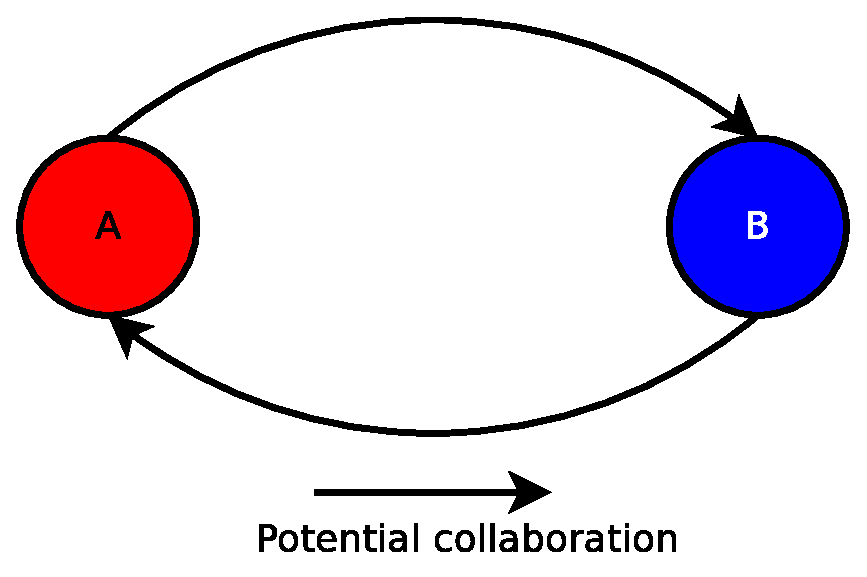
\includegraphics[scale=0.3]{problemDescription/figs/direct-reciprocity.eps}}
	\caption{Direct reciprocity between participants.}
	\label{fig:direct-reciprocity}
\end{figure}

In a large scale, distributed system, this dilemma occurs with every interaction between nodes.
The node can already be familiar with the peer,
but more often the peer will be a peer the node has not interacted with before.
A further complication is that help is one way and can no longer be exchanged.
This complication excludes the direct opportunity to barter for help 
or to barter for help in the future\cite{Lai-Incentives}.
A third complication is that the cooperation node does not incur a penalty for not helping.
The performance of the tit-for-tat or win-stay, lose-shift strategies
quickly deteriorate in such a situation.

For a node it is easier to abuse the generosity of others in this more anonymous situation.
Nodes can act irrational and against the best interest of the network
and this is seen in the real world\cite{Adar-Freeriding}.
Nodes that help others will be penalized through the cost they incur
and incentivized to adopt the malicious behavior themselves.
Nodes in general will become more reluctant to help nodes\cite{Nowak-PrisonerDilemma}.
In the end no node will help another and all nodes will receive a penalty.
This is commonly called the Tragedy of the Commons in the literature \cite{Hardin-Tragedy}.
The whole network will actually receive more benefit in total if everyone would corporate.
But nodes have no way of knowing if the peer they encounter are willing to help.
A lack of altruism and selfishness will become a problem 
and will cause the network to be suspectible to freeriding.

\section{Recording of community contributions}
In the Iterated Prisoner's Dilemma the history of the previous transactions can be used 
to see if a node helped others in the past.
The simple strategies, previously mentioned, uses a history to improve performance
to avoid freeriding.
If a node knows that a history is kept of his previous transactions,
then the node can be fearful of the consequences of his current decision to freeride on public goods.
This is know as the shadow of the future\cite{bo-shadow}.
The shadow of the future can overcome the present current behavior to take advantage of the network.

But this private history is not effective to achieve high overall utility in distributed systems,
because the peers are often interacted with for the first time.
No history is known for these peers.
A public history of a node is necessary to prevent abuse
and is able to achieve high overall utility\cite{Lai-Incentives}.
This public history contains every previous interaction.
The nodes now receive indirect reciprocity\cite{Nowak-Cooperation}.
By helping nodes they will receive help from other nodes in the future based upon their good behaviour.
Indirect reciprocity is displayed abstractly in Figure \ref{fig:indirect-reciprocity}.
The help of node C to node A is dependend on node A helping node B.

\begin{figure}
	\centerline{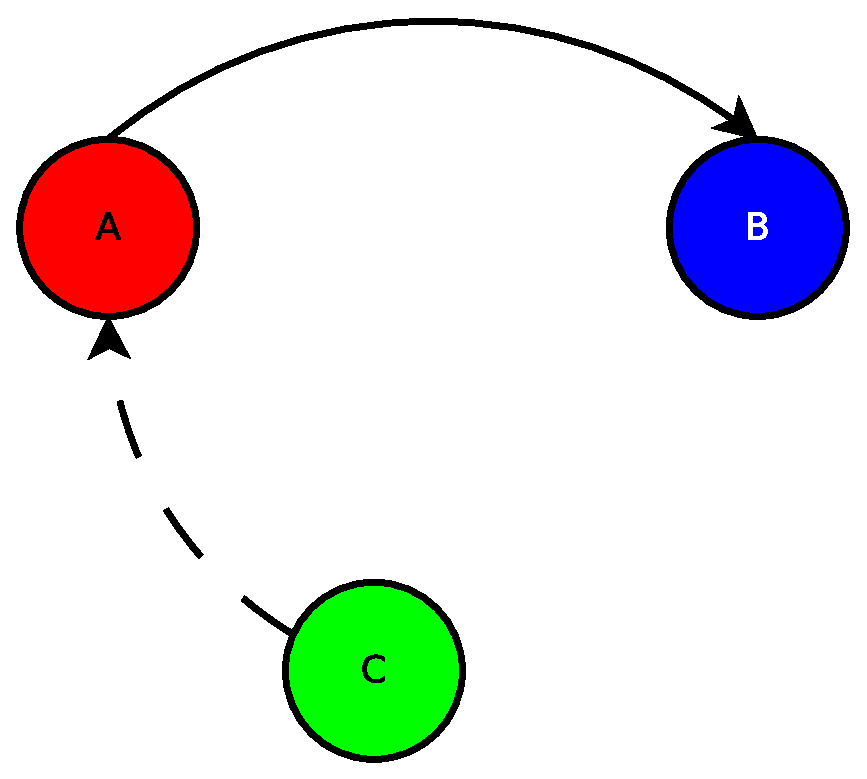
\includegraphics[scale=0.3]{problemDescription/figs/indirect-reciprocity.eps}}
	\caption{Indirect reciprocity between nodes.}
	\label{fig:indirect-reciprocity}
\end{figure}

A history can be used to create a currency or a reputation system
and can be seen as a bookkeeping system.
This history has to be trustworthy.
Here trust is defined as the expectation that the abillity to double spend reputation
or being able to claim a false reputation is highly unlikely.

The node providing help will receive a boost in currency or a beneficial reputation.
The currency or reputation can be used in the future to receive aid.
In a currency system, receiving help will transfer currency to the helper.
In a reputation system, only nodes with a sufficiently good reputation will be helped.

The currency or reputation has to be made publicly available to all nodes in the network.
But a node publicizing to hold a certain reputation is not sufficient as it is not trustworthy.
So a interaction history, that contains every prior interaction a node has conducted, is publicized.
Nodes can cross-reference the interaction history with other nodes and calculate the amount of currency 
or the reputation that a node has.
Based upon this calculation, the node can decide to provide aid or not.

The interaction history has to be distributed among the nodes in the network
to become publicly available.
Efficient distribution protocols are a difficult challenge themselves and outside the problem scope.
But distribution is worth mentioning, because it puts constraints on the interaction history.
The interaction history has to be distributable in an efficient manner.
Only if it meets these constraints, will an interaction history be usable in a distributed system.
The network has to achieve network reciprocity\cite{Nowak-Cooperation}.
Helping peers in the network will ensure that peers themselves receive help.
This is displayed abstractly in Figure \ref{fig:network-reciprocity}.

\begin{figure}
	\centerline{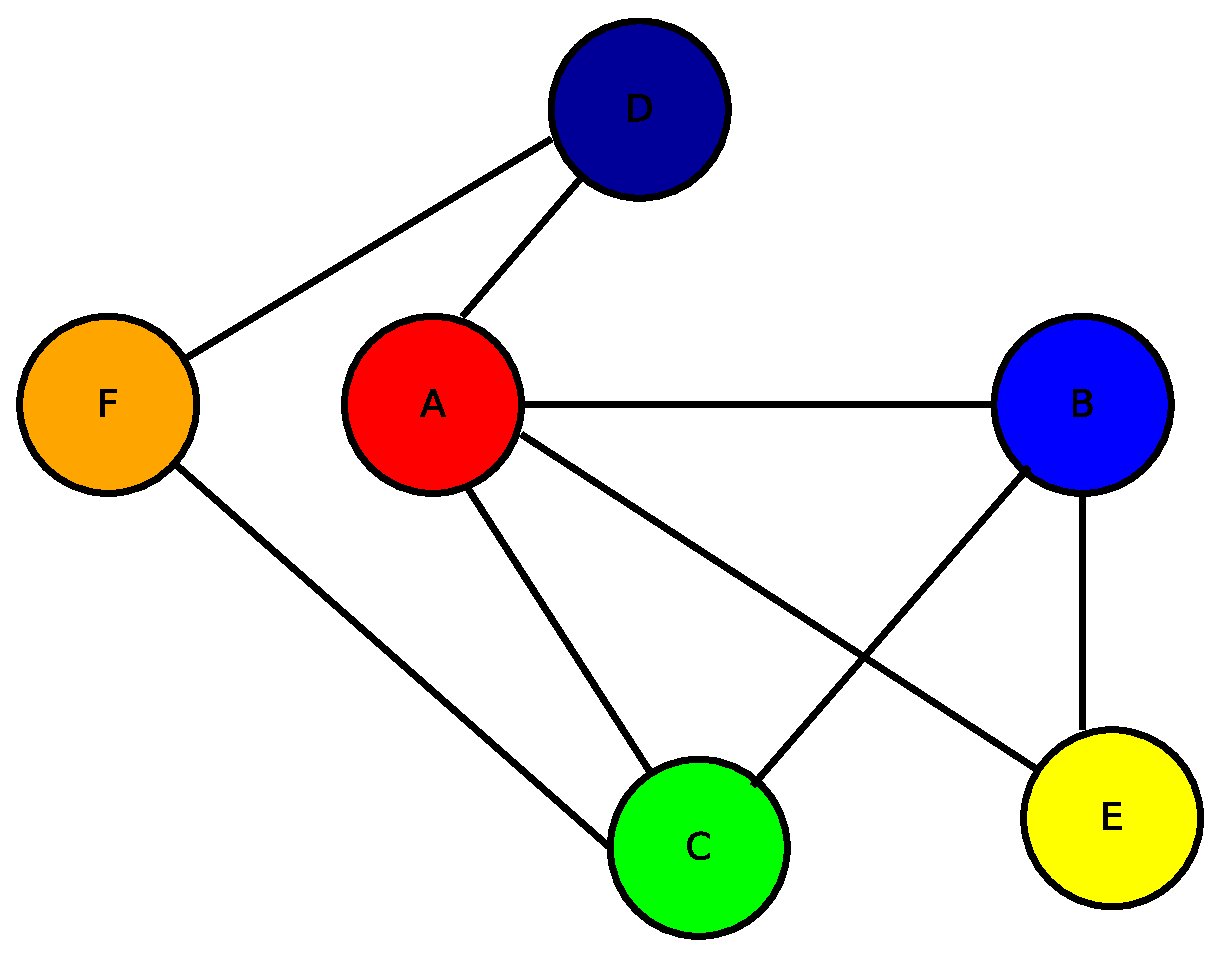
\includegraphics[scale=0.3]{problemDescription/figs/network-reciprocity.eps}}
	\caption{Network reciprocity between nodes.}
	\label{fig:network-reciprocity}
\end{figure}

\section{Facilitating trust}
Interaction histories only prevent direct abuse of the generosity of the nodes.
A malicious node can still try to tamper with the interaction history.
An example of a type of these attacks are double spending attacks\cite{Nakamoto-bitcoin},
where an interaction is altered.
But a node can also try to deny an interaction.
The interaction history has to be resilient to attacks that tamper the interaction history, 
or no one will trust the history. 
A reputation or digital currency system requires a level of trust in the system to function.
The challenge of this thesis is to create a tamper-proof interaction history.

A system cannot be fully secure, 
but still a reasonable certainty can be achieved that no tampering of the interaction history can occur.
Reasonable certainty is for example that no attack can happen 
if more than half of the network consists of honest nodes.

\section{Scalability and no central authority}
\todo{THIS!!}

\section{Aim of this thesis}
\label{pb-aim}
The overall aim of this thesis is to design, implement and conduct experiments with a tamper-proof interaction history
implemented within Tribler.
The interaction history will store a history of the amount of data downloaded between nodes in the network.
This interaction history is cryptographically protected and validated.
In the future this interaction history can be used to decide the level of cooperation with another node in the network.
An incremental approach is taken with this thesis as the first step in creating a fully tamper-proof interaction history.
Several more steps are needed and these steps are explained in chapter \ref{problems}.
